\documentclass[11pt]{article}

\usepackage[margin=1in]{geometry}
\usepackage{setspace}
\usepackage{enumitem}
\usepackage{hyperref}
\usepackage{titlesec}
\usepackage{pdfpages}

\setstretch{1.08}
\setlength{\parindent}{0.25in}
\setlength{\parskip}{0.35em}
\setlist[itemize]{leftmargin=1.4em,itemsep=0.15em,topsep=0.2em}
\titleformat{\section}{\large\bfseries}{\thesection}{0.5em}{}
\titlespacing*{\section}{0pt}{0.8em}{0.35em}

\begin{document}

\begin{center}
{\Large \textbf{Writing Lab Reflection}}\\[0.35em]
EDCI 59100-016: Literature Review\\
Kamrul Md Kamruzzaman\\
Summer 2026
\end{center}

\section*{Coach Report Record}

\textbf{Report source:} Purdue OWL Report email saved from Outlook.\\
\textbf{From:} Purdue OWL \textless noreply@mywconline.com\textgreater\\
\textbf{Date:} Monday, June 15, 2026, 10:30 AM\\
\textbf{To:} Md Kamruzzaman Kamrul \textless mkamrul@purdue.edu\textgreater\\
\textbf{Attachment:} Chapter 1245 Intro method analysis\_v2.docx\\
\textbf{Client:} MD KAMRUZZAMAN KAMRUL\\
\textbf{Staff or resource:} Jacqueline B.\\
\textbf{Appointment date:} June 15, 2026, 10:00 AM - 11:00 AM\\
\textbf{Document type:} Other assignment or essay for class\\
\textbf{Session focus:} Understanding the assignment\\
\textbf{Appointment type:} Regular appointment in Krach Leadership Center

Jacqueline's report note states:

\begin{quote}
Hey MD,

Thank you for sharing your writing with me today. Today, we went over some really well-thought-out questions you had about this methodology. We talked about what types of descriptive analysis would make sense, we talked about the smaller number of papers due to it being such a new topic, and we talked about putting the discussion into one chapter instead of two. Please see the attachment for more details. Overall, I think you're thinking about this really purposefully and well!

Write on,

Jacqueline
\end{quote}

The reviewed draft also included comments that the work was drafted according to PRISMA-ScR and that the paper should be organized around two major sections. In the meeting, I also asked whether my research questions fit the project, and Jacqueline approved the direction of those questions.

\section*{Reflection}

This session helped me clarify the role of Chapter Three in my literature review. I asked specifically what kind of descriptive analysis would be appropriate, and Jacqueline's answer helped me see that I should not treat the chapter like a meta-analysis. Because my topic is new and the studies use different designs, data sources, models, and outcomes, the better approach is to map the field carefully. In my revision, I will describe the number of studies, publication years, countries or regions, journals, publication types, study designs, data sources, sample populations, sample sizes, settings, outcomes, modeling approaches, statistical or machine-learning methods, and any theories or conceptual frameworks used by the studies. This will make the methodology chapter more transparent and better aligned with a PRISMA-ScR scoping review.

The session also helped me make two larger decisions about the structure of the paper. First, Jacqueline confirmed that the smaller number of papers is understandable because VLM-based construction safety and progress monitoring is still an emerging topic; I need to explain that clearly rather than apologizing for it. Second, she advised me not to present findings in two separate chapters. I plan to merge the findings into one chapter so the paper does not repeat the same evidence in different places. My next revision will therefore keep the approved research questions, strengthen the descriptive-analysis and charting plan, and use one findings chapter to present publication patterns, study characteristics, methodological patterns, topic/content patterns, and theoretical grounding in a more organized way.

\clearpage
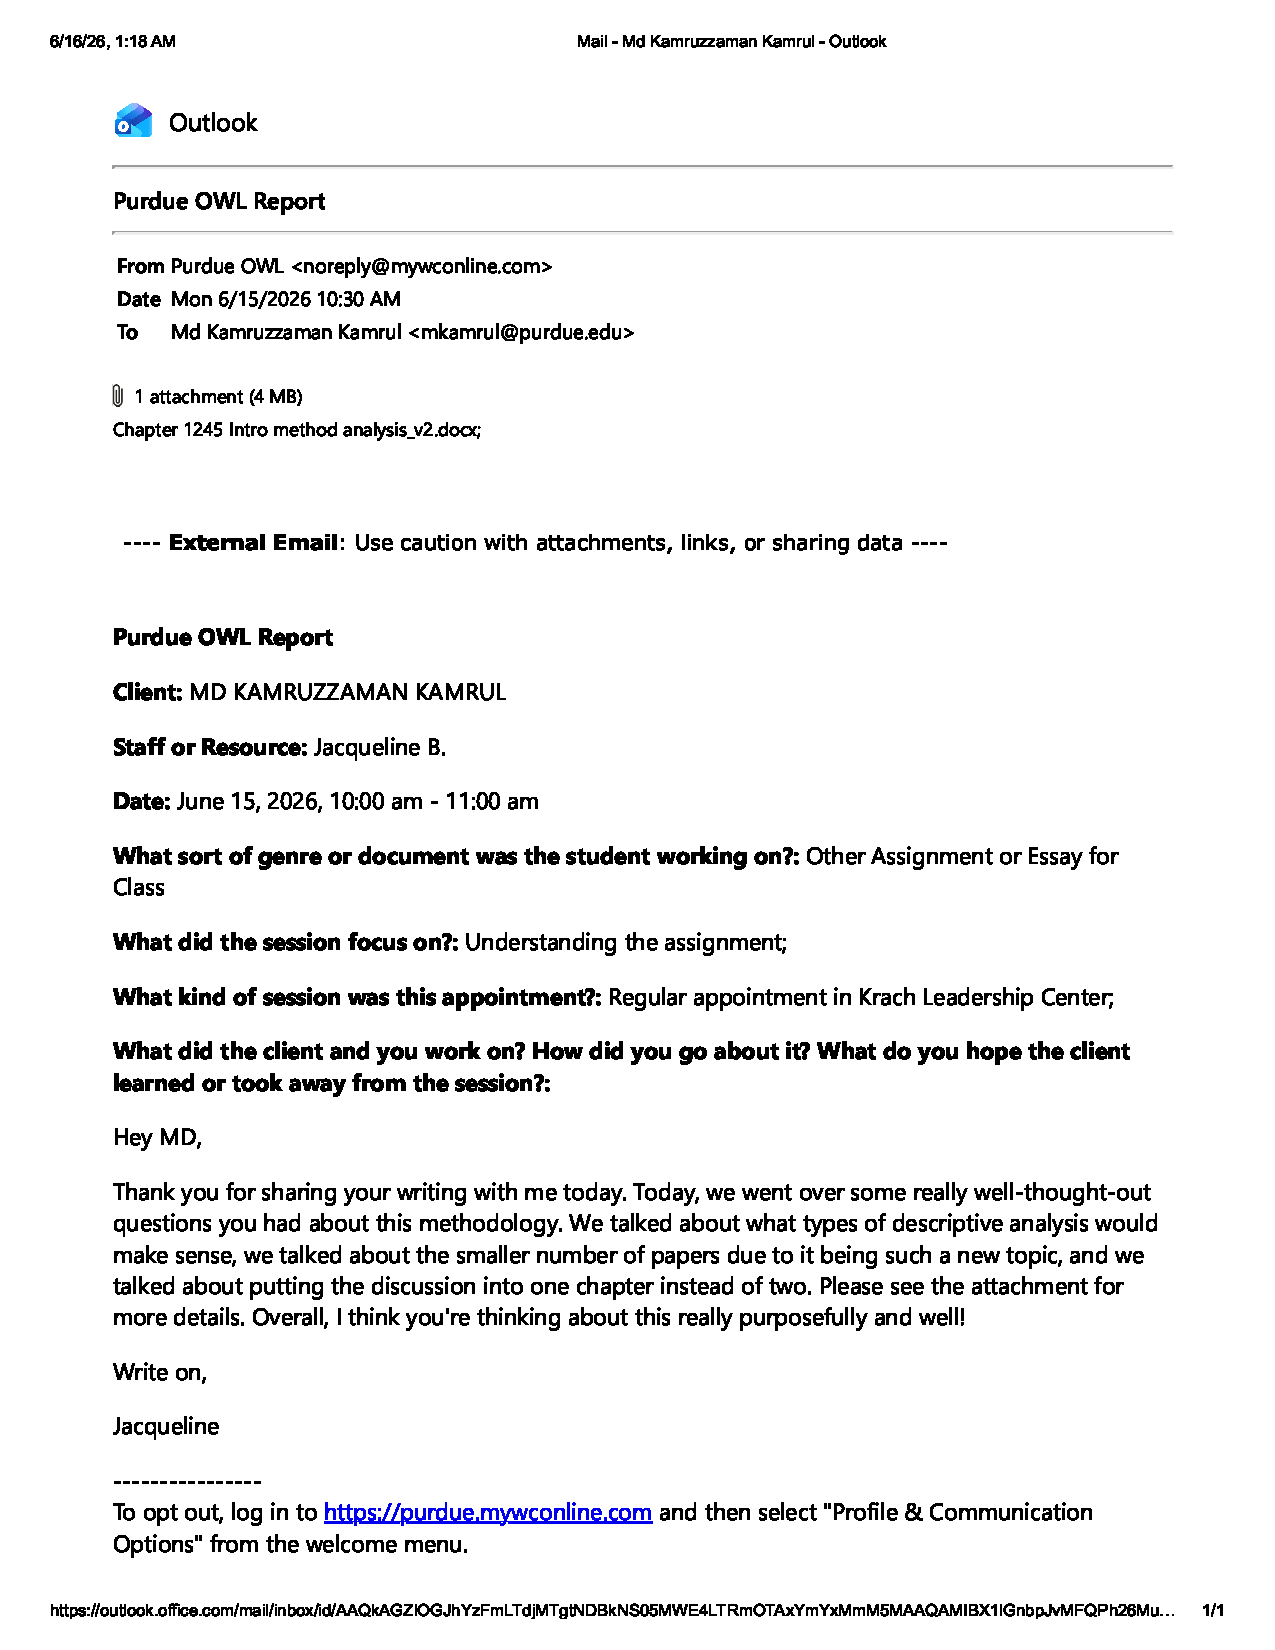
\includepdf[
  pages=-,
  pagecommand={\thispagestyle{plain}},
  scale=0.92
]{Writing_Lab_Email_Report_Outlook.pdf}

\end{document}
